\documentclass[a4paper,11pt]{article}
\pdfoutput=1 % if your are submitting a pdflatex (i.e. if you have
             % images in pdf, png or jpg format)

\usepackage{jcappub} % for details on the use of the package, please
                     % see the JCAP-author-manual

\usepackage[T1]{fontenc} % if needed
\usepackage{eucal}
\usepackage{xspace}
\usepackage{color}

\usepackage[justification=justified]{caption}


\title{ PyUltraLight: A Pseudo-Spectral Solver for Ultralight Dark Matter Dynamics}


%% %simple case: 2 authors, same institution
%% \author{A. Uthor}
%% \author{and A. Nother Author}
%% \affiliation{Institution,\\Address, Country}

% more complex case: 4 authors, 3 institutions, 2 footnotes
\author[]{Faber Edwards,}
\author[]{Emily Kendall,}
\author[]{Shaun Hotchkiss,}
\author[]{and Richard Easther}

% The "\note" macro will give a warning: "Ignoring empty anchor..."
% you can safely ignore it.

\affiliation[]{Department of Physics, University of Auckland, Private Bag 92019, Auckland, New Zealand}


% e-mail addresses: one for each author, in the same order as the authors
\emailAdd{faberedwards@gmail.com}
\emailAdd{eken000@aucklanduni.ac.nz}
\emailAdd{s.hotchkiss@auckland.ac.nz}
\emailAdd{r.easther@auckland.ac.nz}


\newcommand{\apj}{Astrophysical J.}
\newcommand{\prd}{Phys. Rev. D}
\newcommand{\mnras}{Mon. Notices Royal Astron. Soc}
\newcommand{\PyUltraLight}{\textsc{PyUltraLight}\xspace}
\newcommand{\re}[1]{\textcolor{blue}{[{\bf RE}: #1]}}

\abstract{\PyUltraLight  simulates the dynamics of ultralight dark matter in a static, non-expanding background.  \PyUltraLight can describe the evolution of several interacting ultralight dark matter halos  or one or more halos orbiting a central, fixed Newtonian potential, the latter scenario corresponding to dwarf galaxies orbiting a massive central galaxy. We verify  \PyUltraLight  by showing that it reproduces qualitative dynamical features of previously published simulations and demonstrate that it has  excellent energy-conservation properties.   \PyUltraLight is implemented in a Python-based Jupyter notebook, solving the Schr{\"o}dinger-Poisson equation  governing  ultralight scalar field dark matter dynamics in the non-relativistic regime using a symmetrised split-step pseudospectral  algorithm. The notebook interface makes it simple to specify simulation parameters and  visualise the resulting output. \PyUltraLight  runs on standard desktop hardware and is available on GitHub.  }




\begin{document}
\maketitle
\flushbottom

\section{Introduction}
\label{sec:intro}

The realisation that there may be more to the universe than meets the eye is one of the most profound developments in 20$^{\textrm{th}}$ Century astronomy and astrophysics. However, while there are now multiple lines of evidence that dark matter outweighs baryonic matter by a ratio of approximately 5:1 \cite{Planck2015}, we have few clues regarding the physical nature of dark matter.  Much theoretical and experimental effort has focused on  WIMP models, motivated by their consistency with supersymmetric extensions to the Standard Model and their relatively simple dynamics. However, advanced direct-detection experiments are putting increasingly tight constraints on the WIMP parameter space \cite{Tan2016, Akerib2017} and $\Lambda$CDM cosmology with simple, pressureless, noninteracting dark matter (a class including simple WIMP scenarios) is potentially at odds with observations at small astrophysical scales \cite{Bull2016}.  

The potential shortcomings of simple cold dark matter scenarios motivate investigations of more novel dark matter scenarios. In particular, ultralight dark matter (ULDM), also known as fuzzy dark matter (FDM), or BEC dark matter, is an increasingly well-studied possibility; for a recent review of the potential advantages and characteristic attributes of this scenario see Ref~\cite{Hui2016}.   ULDM models are well motivated by fundamental theories possessing approximate shift symmetries. Moreover, ULDM can naturally resolve the small-scale problems of $\Lambda$CDM as the Heisenberg uncertainty principle suppresses gravitational collapse on length scales shorter than the de Broglie wavelength of the ULDM particle. In this regime the mass of the ULDM particle becomes correlated with astrophysical observables; if it is on the order of $10^{-22}$~eV, structure is suppressed at kiloparsec scales and below \cite{Hu2000}. 


Given the presence of a fundamental  lengthscale, the behaviour of ULDM is more complex than that of simple dark matter scenarios whose cosmologically relevant interactions are purely gravitational. Physically, the effective short-scale pressure and  condensate-like properties of ULDM  create new dynamical possibilities for ULDM scenarios, such as  purely pressure supported soliton-like solutions  \cite{Marsh2015} and superposition or interference during interactions between condensate-like halos \cite{Schwabe2016}. Consequently, modelling dark matter dynamics in ULDM scenarios is more challenging than in simple cold dark matter models, but is critical to understanding the physical consequences of ULDM models. 

In the non-relativistic regime, the dynamics of ULDM can be reduced to the Schr{\"o}dinger-Poisson  system, where the complex variable $\psi$ describes the local density of ULDM quanta while the Poisson equation describes the local gravitational potential. Many approaches have been taken to this problem, including both modifications of existing cosmological simulation codes and the development of new codes specifically designed for ULDM systems. One widely used approach is the Madelung fluid formulation of the Schr{\"o}dinger-Poisson system \cite{Madelung1926} which has a quantum pressure term that can be treated numerically in a variety of ways. In Ref.~\cite{Zhang2018}, the cosmological code \textsc{gadget} \cite{Springel2005} is modified to treat the quantum pressure as an effective particle-particle interaction and the resulting code, \textsc{axion-gadget} is publicly available \cite{axion-gadget}.  Ref.~\cite{Nori2018} modifies a non-public extension of \textsc{gadget}, \textsc{p-gadget3} to treat the quantum pressure term via smoothed-particle hydrodynamics (SPH) routines. The SPH approach is also  used in Ref.~\cite{Mocz2015}, while a particle-mesh approach was implemented in \cite{Veltmaat2016}. N\textsc{yx} \cite{Almgren2013} was modified in \cite{Schwabe2016} to study merging ULDM solitonic cores, G\textsc{alacticus} \cite{Benson2012} was modified in \cite{Du2017} to study the effects of tidal stripping and dynamical friction on ULDM halos, \textsc{arepo} \cite{Springel2010} was modified in \cite{Mocz2017} to study the core-mass relationship and turbulence characteristics of ULDM halos, and \textsc{gamer} \cite{Schive2010, gamer} was modified \cite{Schive2014_b} to perform a detailed study of structure formation in ULDM cosmologies. 

While a large number of public codes can solve conventional dark matter scenarios, \textsc{axion-gadget} is the only currently available solver for ULDM dynamics. This paper introduces \PyUltraLight, a stand-alone Python-based pseudospectral Schr{\"o}dinger-Poisson solver, and  demonstrates that it reproduces many of the key findings of more complicated cosmological simulation codes within a desktop computing environment. We anticipate that as a publicly available resource, \PyUltraLight\ will serve as a valuable cross-check on more complex implementations, serve as a basis for further development of such codes within the computational cosmology community, and facilitate explorations of ULDM dynamics.   

\PyUltraLight is based on a symmetrised-split-step (leapfrog) solver for the time evolution, and uses a pseudospectral Fourier algorithm to solve the Poisson equation for the gravitational potential at each step.\footnote{A similar methodology was described in Ref.~\cite{Paredes2016}; to our knowledge this code has not been released.} This algorithm has $2^{nd}$ order accurate time integration steps and sub-percent level energy conservation, while the wavefunction normalisation  is conserved to machine precision. As a pseudospectral code, linear differential operators are computed by direct multiplication in the Fourier domain, while non-linear terms are evaluated in position space. Consequently, \PyUltraLight is free from noise associated with spatial derivatives computed via finite-differencing. There is a necessary computational cost associated with the Fourier and inverse Fourier transforms but these transforms are optimised in \PyUltraLight\ through the use of the pyFFTW pythonic wrapper around the C-based FFWTW subroutine library \cite{pyfftw,fftw}. \PyUltraLight is currently takes advantage of multiple cores on a singe machine but the FFTW libraries offer full parallelisation, so there is no barrier to running the code in a cluster environment. \re{ Will the ``top level" Python routines run in a full MPI environment; i.e. a cluster based shared-memory implementation? We would need this to make the full cluster-based approach work.}

This paper is organised as follows. We first provide a short review of ULDM physics, including a derivation of the Schr{\"o}dinger-Poisson equations from the underlying scalar-field Lagrangian. We then describe their implementation in \PyUltraLight, before moving on to the testing and verification Section in which we reproduce a selection of results from a variety of recent ULDM simulations and discuss energy conservation within the code. 


\section{The Physics of ULDM}\label{sec:physics}

\subsection{The Schr{\"o}dinger-Poisson System}

The existence of an extremely light scalar field, minimally coupled to gravity, is the central premise on which ULDM models are predicated. Within the ULDM framework, it is proposed that cosmological structure formation proceeds through the Bose-Einstein condensation of this scalar field. In this Section  \re{I would nornally give Section a capital letter in this context} we derive the (non-relativistic) dynamical equations of the single macroscopic condensate wavefunction, namely, the Schr{\"o}dinger-Poisson equations. We begin with the action functional for a scalar field, $\phi$, minimally coupled to gravity and in the absence of self-interactions,
%
\begin{equation}\label{eq:action}
    S=\int \frac{d^4x}{\hbar}\sqrt{-g}\bigg\{\frac{1}{2}g^{\mu\nu}\partial_\mu\phi\partial_\nu\phi-\frac{m^2}{2\hbar^2}\phi^2\bigg\},
\end{equation}
%
where we have taken $c=1$ but retain factors of $\hbar$ at this stage. Applying the variational principle to this action yields the Euler-Lagrange equations
%
\begin{equation}\label{eq:e-l}
    \frac{1}{\sqrt{-g}}\partial_\mu\big[\sqrt{-g}g^{\mu\nu}\partial_\nu\phi\big]-\frac{m^2}{\hbar^2}\phi=0.
\end{equation}
We evaluate equation \ref{eq:e-l} using linear perturbation theory, adopting the perturbed FRW metric in the Newtonian gauge:
\begin{equation}\label{eq:pFRW}
    ds^2=-\big(1+2\Phi(\vec{r})\big)dt^2+a(t)^2\big(1-2\Phi(\vec{r})\big)d\vec{r}^{\,2}.
\end{equation}
To linear order in $\Phi(\vec{r})$ we obtain 
\begin{equation}\label{eq:linear}
    \Ddot{\phi}-\frac{\big(1+4\Phi(\vec{r})\big)}{a(t)^2}\nabla^2\phi+3\big(1+2\Phi(\vec{r})\big)H\Dot{\phi}+\big(1+2\Phi(\vec{r})\big)\frac{m^2}{\hbar^2}\phi=0,
\end{equation}
where $H=\Dot{a}(t)/a(t)$. We will work in the limit $H\ll m$ and it is sufficient to set $H=0$ and $a(t)=1$ in equation \ref{eq:linear}. \footnote{ \re{ Just checking -- we could say we were working in a  non-expanding universe and just set $H=0$ whatever $m$ was?  Physically, what does this statement mean? Can we say when this approximation becomes good for $m=10^{-22}$eV dark matter? We go on to say non-relativistic, but is that synonymous with non-expanding?}}  In the non-relativistic limit,  the WKB approximation gives an ansatz for a  solution to equation \ref{eq:linear}.  We take 
\begin{equation}\label{eq:ansatz}
    \phi=\frac{\hbar}{\sqrt{2}m}\big(\psi e^{-imt/\hbar}+\psi^* e^{imt/\hbar}\big),
\end{equation}
where $\psi$ is assumed to be slowly varying (with respect to intervals $\Delta t\sim \hbar/m$ \re{right?}) complex function so that terms involving $\Ddot{\psi}$ may be neglected. We may also use $\nabla^2\phi\ll m^2/\hbar^2\phi$, \re{physical origin of this} such that our final result takes the form
\begin{equation}\label{eq:schrodinger}
    i\hbar\Dot{\psi}=-\frac{\hbar^2}{2m}\nabla^2\psi+m\Phi\psi.
\end{equation}
We have thus show that $\psi$ satisfies the Schr{\"o}dinger equation in this limit, which is interpreted as the unique macroscopic wavefunction of a Bose-Einstein condensate. It follows that the particle density of the condensate is given by $\vert\psi\vert^2$, so its mass density is simply $m\vert\psi\vert^2$. The local gravitational potential thus satisfies the Poisson equation,
\begin{equation}\label{eq:poisson}
    \nabla^2\Phi=4\pi G m \vert\psi\vert^2,
\end{equation}
where $G$ is Newton's gravitational constant. The coupled equations \ref{eq:schrodinger} and \ref{eq:poisson} together form the nonlinear Schr{\"o}dinger-Poisson system which describes the dynamics of ULDM in the non-relativistic regime. It is this system of equations which \PyUltraLight is designed to solve. \re{I try to avoid acronyms like SP; ULDM works since it replaces something very long, and CDM is common usage, but I think papers are more readable if they are used sparingly}


\subsection{Field Rescalings}

It is helpful to recast the Schr{\"o}dinger-Poisson system (equations \ref{eq:schrodinger} and \ref{eq:poisson}) in terms of adimensional quantities. In keeping with Refs~\cite{Schive2014,Paredes2016} we introduce length, time, and mass scales as follows:
\begin{align}
    \CMcal{L}&=\left(\frac{8\pi\hbar^2}{3 m^2H_0^2\Omega_{m_0}}\right)^{\frac{1}{4}}\approx121\left(\frac{10^{-23}\operatorname{eV}}{m}\right)\operatorname{kpc},\label{eq:length}\\
    \CMcal{T}&=\left(\frac{8\pi}{3 H_0^2\Omega_{m_0}}\right)^{\frac{1}{2}}\approx75.5 \operatorname{Gyr},\label{eq:time}\\
    \CMcal{M}&=\frac{1}{G}\left(\frac{8\pi}{3 H_0^2\Omega_{m_0}}\right)^{-\frac{1}{4}}\left(\frac{\hbar}{m}\right)^{\frac{3}{2}}\approx 7\times 10^7\left(\frac{10^{-23}\operatorname{eV}}{m}\right)\operatorname{M}_{\odot},\label{eq:mass}
\end{align}
where $m$ is the mass of the ultralight scalar field, $H_0$ is the present-day Hubble parameter, $G$ is Newton's gravitational constant and $\Omega_{m_0}$ is the present-day matter fraction of the energy density of the universe. We  recast equations \ref{eq:schrodinger} and \ref{eq:poisson} in terms of the  dimensionless quantities
\begin{equation}\label{eq:dimensionless}
    t'=\frac{t}{\CMcal{T}},\quad
    \vec{x}^{\,'}=\frac{\vec{x}}{\CMcal{L}},\quad
    \Phi'=\frac{m\CMcal{T}}{\hbar}\Phi,\quad
    \psi'=\CMcal{T}\sqrt{mG}\psi.
\end{equation}
Dropping the primes for notational convenience, we see that the coupled differential equations of the  Schr{\"o}dinger-Poisson system  reduce to 
\begin{align}
    i\Dot{\psi}(\vec{x},t)&=-\frac{1}{2}\nabla^2\psi(\vec{x},t)+\Phi(\vec{x},t)\psi(\vec{x},t),\label{eq:s-adim}\\
    \nabla^2\Phi(\vec{x},t)&=4\pi\vert\psi(\vec{x},t)\vert^2,\label{eq:p-adim}
\end{align}
where it is understood that all quantities involved are dimensionless. We can recover  dimensionful quantities via the ``dictionary'' provided by equations \ref{eq:length} to \ref{eq:mass}. For example, the integrated mass of the system, $M_{tot}$, is given by
\begin{equation}\label{eq:integrated-mass}
    M_{tot}=\CMcal{M}\int d^3x\vert\psi\vert^2.
\end{equation}
Likewise, the mass density at any point is given by
\begin{equation}\label{eq:density}
    \rho=\frac{\CMcal{M}}{\CMcal{L}^3}\vert\psi\vert^2.
\end{equation}
\PyUltraLight\ works internally with these dimensionless quantities but receives initial conditions and generates output in physical units. Henceforth, we will often refer to $\vert\psi\vert^2$  as the density, where it is understood that this is in fact a dimensionless quantity related to the physical mass density via the constant of proportionality given by equation \ref{eq:density}.




\section{Algorithm and Implementation}\label{sec:implementation}

In this section we discuss the methodology used to calculate the dynamics of the adimensional  Schr{\"o}dinger-Poisson system (equations \ref{eq:s-adim} and \ref{eq:p-adim}) given user-specified initial conditions. We introduce the symmetrised split-step Fourier method, and schematically describe  how the system is evolved at each timestep. 

\subsection{Dynamical Evolution}\label{sec:dynamics}

Dynamical evolution within \PyUltraLight\ progresses via a symmetrised split-step Fourier process on an $N\times N\times N$  grid with  periodic spatial boundary conditions. To understand this method,  first consider the exact expression for the unitary time evolution of the wavefunction according to equation \ref{eq:s-adim}, namely
\begin{equation}\label{eq:exact-time-ev}
    \psi(\vec{x},t+h)=\mathcal{T}\operatorname{exp}\left[-i\int_t^{t+h}dt'\left\{-\frac{1}{2}\nabla^2+\Phi(\vec{x},t')\right\}\right]\psi(\vec{x},t),
\end{equation}
where $\mathcal{T}$ is the time-ordering symbol. For a sufficiently small timestep $h$,  the trapezoidal rule gives the approximation
\begin{equation}
    \int_t^{t+h}dt'\Phi(\vec{x},t')\approx \frac{h}{2}\Big(\Phi(\vec{x},t\hspace*{-.2em}+\hspace*{-.2em}h)+\Phi(\vec{x},t)\Big).
\end{equation}
We can therefore write the approximate form of equation \ref{eq:exact-time-ev} as
\begin{equation}\label{eq:approx-time-ev}
    \psi(\vec{x},t+h)\approx \operatorname{exp}\left[i\frac{h}{2}\Big(\nabla^2-\Phi(\vec{x},t\hspace*{-.2em}+\hspace*{-.2em}h)-\Phi(\vec{x},t)\Big)\right]\psi(\vec{x},t).
\end{equation}
Note that the exponential in equation \ref{eq:approx-time-ev} omits the time-ordering symbol, and is only equivalent to its time-ordered counterpart to order $h^2$. \re{to here}

The linear differential operator in equation \ref{eq:approx-time-ev} acts naturally in Fourier space, while the nonlinear potential term is simplest to evaluate in position space and by splitting the exponential we can evaluate each term in its natural domain.  For small timesteps we assume that the dispersive and nonlinear terms act independently,  adopting the specific evolution scheme  
%
\begin{equation}\label{eq:split-step}
    \psi(\vec{x},t\hspace*{-.2em}+\hspace*{-.2em}h)\approx\operatorname{exp}\left[-\frac{ih}{2}\Phi(\vec{x},t\hspace*{-.2em}+\hspace*{-.2em}h)\right]\operatorname{exp}\left[\frac{ih}{2}\nabla^2\right]\operatorname{exp}\left[-\frac{ih}{2}\Phi(\vec{x},t)\right]\psi(\vec{x},t).
\end{equation}
%
This splitting can be understood thusly: first, a half timestep is taken in which only the nonlinear potential operator acts, followed by a full timestep in the linear term. The potential field is then updated, and a final half timestep in the nonlinear term is performed. Using the Baker-Campbell-Hausdorff formula to express the product of exponentials in equation \ref{eq:split-step} as a single exponential and keeping only terms to order $h^2$ we find:
\begin{equation}\label{eq:BCH}
    \operatorname{exp}\left[i\frac{h}{2}\Big(\nabla^2-\Phi(\vec{x},t\hspace*{-.2em}+\hspace*{-.2em}h)-\Phi(\vec{x},t)\Big)+\frac{h^2}{8}\Big[\nabla^2,\Phi(\vec{x},t)\Big]-\frac{h^2}{8}\Big[\nabla^2,\Phi(\vec{x},t\hspace*{-.2em}+\hspace*{-.2em}h)\Big]\right].
\end{equation}
Making use of the fact that $\Phi(\vec{x},t+h)\approx\Phi(\vec{x},t)+h\Dot{\Phi}(\vec{x},t)$ we see that the commutators in equation \ref{eq:BCH} cancel at $\mathcal{O}(h^2)$ and the expression matches \ref{eq:approx-time-ev}, with the dominant error term appearing at $\mathcal{O}(h^3)$. 

Evaluation of equation \ref{eq:split-step} within \PyUltraLight thus proceeds as follows:
Initially, the nonlinear term acts in position space for one half-timestep. The result is  Fourier transformed, and a full timestep is taken with the differential operator  applied in the Fourier domain. The potential field is then updated in accordance with equation \ref{eq:p-adim}. After an inverse Fourier transform a final half timestep is taken with the updated nonlinear term acting in position space to give the new $\psi$ field configuration. This procedure is known as the symmetrised split-step Fourier method, and  used widely in fields such as nonlinear fiber optics \cite{Agrawal2013}. \re{do we want a couple of other examples/cites?} 

The algorithm can be represented schematically as
\begin{equation}\label{eq:schematic-psi}
    \psi(\vec{x},t\hspace*{-.2em}+\hspace*{-.2em}h)=\operatorname{exp}\left[-\frac{ih}{2}\Phi(\vec{x},t\hspace*{-.2em}+\hspace*{-.2em}h)\right]\CMcal{F}^{-1} \operatorname{exp}\left[\frac{-ih}{2}k^2\right]\CMcal{F}\operatorname{exp}\left[-\frac{ih}{2}\Phi(\vec{x},t)\right]\psi(\vec{x},t),
\end{equation}
where the order of operations runs from right to left, $\CMcal{F}$ and $\CMcal{F}^{-1}$ denote the discrete Fourier transform and its inverse, and $k$ is the wavenumber in the Fourier domain. The potential field is updated following the inverse Fourier transform in equation \ref{eq:schematic-psi}, via
%
\begin{equation}\label{eq:schematic-phi}
    \Phi(\vec{x},t\hspace*{-.2em}+\hspace*{-.2em}h)=\CMcal{F}^{-1}\left(-\frac{1}{k^2}\right)\CMcal{F}\ 4\pi\vert\psi(\vec{x},t_{i})\vert^2,
\end{equation}
%
where $\psi(\vec{x},t_{i})$ is the field configuration at this halfway point in the full timestep. The final operation in equation \ref{eq:schematic-psi}  only changes the phase of  $\psi$, so we could replace $\psi(\vec{x},t_{i})$ with $\psi(\vec{x},t\hspace*{-.2em}+\hspace*{-.2em}h)$ in equation \ref{eq:schematic-phi} with no change in meaning. \PyUltraLight makes an additional simplification ti the symmetrised split-step Fourier method as the consecutive half-steps in the nonlinear term may be combined into a single full step. Consequently, only the first and last operations involve actual half steps. Schematically this becomes 
%
\begin{equation}
    \psi(t\hspace*{-.2em}+\hspace*{-.2em}nh)=\operatorname{exp}\left[+\frac{ih}{2}\Phi\right]\left(\prod^n\operatorname{exp}\left[-\frac{ih}{2}\Phi\right]\operatorname{exp}\left[\frac{ih}{2}\nabla^2\right]\right)\operatorname{exp}\left[-\frac{ih}{2}\Phi\right]\psi(t),
\end{equation}
%
where  $\Phi$  is updated at each step via equation \ref{eq:schematic-phi}; attention is drawn to the sign difference between the first and last operators.


From a computational perspective, the numerical Fourier transforms are likely to be rate-limiting step in any pseudospectral code. In \PyUltraLight the discrete Fourier transform (DFT) and its inverse are implemented via pyFFTW, a pythonic wrapper for the C-based FFTW subroutine library which efficiently implements both real and complex DFTs \cite{pyfftw,fftw,Frigo2005}. This  allows  \PyUltraLight  to combine the flexibility of a notebook based modelling tool with the efficiency of a carefully tuned, compiled numerical library.  FFTW is fully parallelised and its support for multithreading  is inherited  by pyFFTW and accessed within \PyUltraLight; the number of threads used by the pyfftw.FFTW class is determined by the  Python multiprocessing routines which are used to ascertain the number of available CPU cores. In addition, \PyUltraLight uses the NumExpr package to parallelise operations on array objects within the simulation \cite{numexpr}. 

\subsection{Initial Conditions: Soliton Profiles}\label{sec:soliton-profiles}

\PyUltraLight specifies the initial dark matter configuration as a superposition of an arbitrary number of solitonic halos, with arbitrary (user-defined) velocities and phases. This is necessarily an idealisation, given that realistic dark matter halos will not map directly to the solitonic solutions, but it provides an excellent ``playground'' in which to explore ULDM dynamics, and the initialisation routines within \PyUltraLight can be easily augmented to accommodate a wider range of scenarios. The initial field configuration is built by loading a NumPy array file encoding a solitonic solution to the Schr{\"o}dinger-Poisson system and the corresponding position mass, velocity, and phase parameters each specified by the user within the accompanying Jupyter notebook. 

In practice, only a finite  range of halo masses can be supported within a given simulation -- the  radius of a solitonic halo is inversely proportional to its mass, so resolving a light halo interacting with a very massive halo would require an extremely fine spatial mesh.  However, \PyUltraLight also allows the user to specify a fixed, external potential which does not take part in the dynamics. At this point only a central $1/r$ potential is supported but this would be easily generalised. \re{new material. Also, do we need to say anything about what happens when the solitions cross into the ``next" box?}
 
The soliton profile is found by imposing a spherically symmetric profile \cite{Paredes2016} where the radial profile is assumed to be time independent
%
\begin{equation}
    \psi(\vec{x},t)\rightarrow e^{i\beta t} f(r), \quad \Phi(\vec{x},t)\rightarrow \varphi(r),
\end{equation}
where $r=\vert\vec{x}\vert$. Introducing $\tilde{\varphi}(r):=\varphi(r)+\beta$, equations \ref{eq:s-adim} and \ref{eq:p-adim}  reduce to
\begin{align}
    0 &= -\frac{1}{2}f^{\prime\prime}(r)-\frac{1}{r}f^\prime(r)+\tilde{\varphi}(r)f(r)\label{eq:s-spherical}\\
    0 &= \tilde{\varphi}^{\prime\prime}(r)+\frac{2}{r}\tilde{\varphi}^\prime(r)-4\pi f(r)^2\label{eq:p-spherical}
\end{align}
%
where primes denote derivatives with respect to $r$. Note that this system contains no arbitrary constants, so the underlying profile will effectively be universal and \PyUltraLight loads a precomputed profile supplied with the code, rather than computing it from scratch each time the code is run. However, an auxiliary program {\sc soliton\texttt{\_}solution.py} is supplied with  \PyUltraLight; it uses a  fourth-order Runge-Kutta algorithm to solve the coupled profile equations. We set $\left. f(r) \right|_{r=0}$=1, while  smoothness requires that first derivatives of $f(r)$ and $\tilde{\varphi}(r)$ vanish at the origin. We then use the shooting method to search for solutions of $f(r)$ and $\varphi(r)$  satisfying the boundary conditions $\lim_{r\rightarrow\infty}\varphi(r)=0$ and $\lim_{r\rightarrow\infty}f(r)=0$, varying $\left. \tilde{\varphi}(r)\right|_{r=0}$ until we obtain a solution of $f(r)$ which approaches zero at the maximal specified radius, $r_m$. The value of $\beta$ is then calculated by assuming that $\varphi(r)$ goes as $-c/r$ at large radii, where $c$ is a constant. Under this assumption, we can write
\begin{equation}
    \tilde{\varphi}(r_m)=-\frac{c}{r_m}+\beta, \quad c=r_m^2\tilde{\varphi}^{\ \prime}(r_m).
\end{equation}
We thus obtain the full solution $\psi(\vec{x},t)=e^{i\beta t}f(r)$.
Having initially chosen $\left. f(r)\right|_{r=0}=1$, we may then generalise to $\left. f(r)\right|_{r=0}=\alpha$, where $\alpha$ is an arbitrary positive real number. It is easily verified that if $e^{i\beta t}f(r)$ is a solution to the spherically symmetric Schr{\"o}dinger-Poisson system, then $g(r)$ is also a solution, where
\begin{equation}
    g(r)=e^{i\alpha\beta t}\alpha f(\sqrt{\alpha}\ r).
\end{equation}
We thus have a family of spherically symmetric soliton solutions to the dimensionless Schr{\"o}\-dinger-Poisson system; the dimensionless soliton mass is proportional to $\sqrt{\alpha}$ and the full width at half maximum is proportional to $1/\sqrt{\alpha}$. Since the size of the soliton scales inversely with the mass, the most massive soliton in the solution  puts a lower bound on the required spatial resolution. 

The Schr{\"o}dinger equation is not trivially form invariant under Galilean boosts but we can enforce Galilean covariance through the addition of a velocity-dependent phase factor,
%
\begin{equation}\label{eq:covariant-solution}
    \psi(\vec{x},t)=\alpha f\big(\sqrt{\alpha}\vert\vec{x}-\vec{v}t\vert\big)e^{i\left(\alpha\beta t+\vec{v}\cdot\vec{x}-\frac{1}{2}\vert\vec{v}\vert^2t\right)}.
\end{equation}
%
To construct the initial field configuration,  \PyUltraLight, loads the NumPy array encoding the radial profile $f(r)$ for the $\left. f(r)\right|_{r=0}=1$ case. Equation \ref{eq:covariant-solution} is then used to transform the this solution into soliton(s) with user-specified values position, mass, and velocity specified, via the accompanying Jupyter notebook. The user may also add an additional constant phase factor if desired.

\subsection{Timestep Constraints}

In many finite-differencing schemes for  partial differential equations the Courant-Friedrichs-Lewy (CFL) condition is a necessary condition for convergence \cite{Ajaib2013}, and puts an upper bound on the timestep as  function of the gridsize whose physical origin is the finite speed of propagating information  in the evolving system.  Consequently, this condition is often cited in numerical analysis of ULDM physics governed by the Schr{\"o}dinger-Poisson system, see e.g. Ref.~\cite{Schwabe2016}. Strictly speaking, however, the CFL condition is applicable to codes using finite differencing methods for spatial derivatives, and is thus not applicable to pseudospectral codes like \PyUltraLight.   We also note that the Poisson equation is acausal in that it responds globally and instantaneously to local changes in the matter distribution. However, the Schr{\"o}dinger-Poisson equation is an approximation derived  in the nonrelativistic limit so this is not a shortcoming in regimes where the underlying equations are physically valid. 

In place of the CFL condition, the \PyUltraLight timestep can be set via the fluid interpretation of the Schr{\"o}dinger-Poisson system. In dimensionless code units we can write 
\begin{equation}
    \psi\equiv\sqrt{\rho}e^{i\theta}, \quad \vec{v}\equiv\boldsymbol{\nabla}\theta.
\end{equation}
We define a `maximum velocity' for the simulation grid at which point the fluid appears to move backward because the phase change between successive grid points exceeds $\pi$. An upper bound can then be placed on the timestep so that a fluid travelling at this maximum  velocity  traverse a distance of one grid space per timestep.  In practice this can yield a very demanding constraint on the timestep and for many scenarios the actual velocity is far less than this hypothetical limit. Consequently, the timestep can be  significantly increased at the user's discretion but convergence testing on a case-by-case basis is strongly encouraged.


\section{ULDM Dynamics with \PyUltraLight}\label{sec:test}

In this section we validate \PyUltraLight a by reproducing results from previous studies of ULDM dynamics, demonstrating interference effects and effective repulsive forces arising from the wavelike nature of ULDM. In addition we study the evolution of the velocity field of a solitonic core orbiting within a Newtonian central potential, showing that the stable orbital configuration is an irrotational Riemann-S ellipsoid. Finally, we show demonstrate that \PyUltraLight delivers sub-percent level energy conservation for a selection of dynamical scenarios.

\subsection{Interference Patterns During Soliton Collisions}\label{sec:interference}


\begin{figure}
  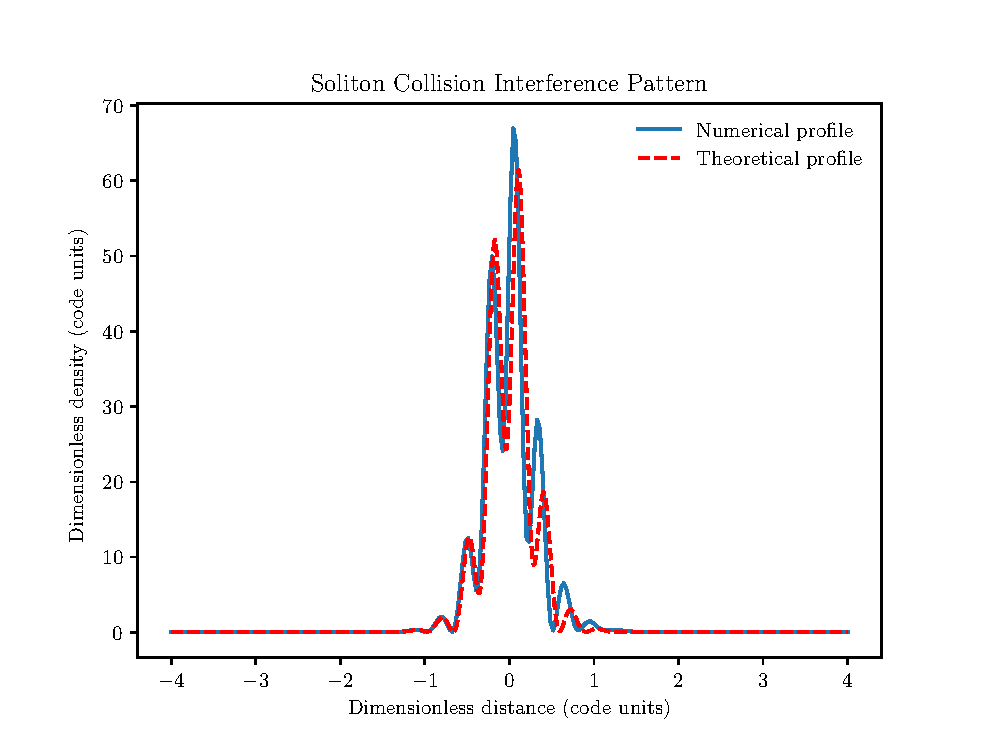
\includegraphics[trim={0 0 0 0.9cm},clip, scale=0.9]{interference_patterns}
  \caption{Comparison of theoretical and numerical density profiles at time of maximal interference for head-on collision of two solitons with mass ratio $\mu=2$ and no relative phase difference. The solitons were chosen with dimensionless masses 5 and 10, with an initial separation of 4 code units and relative velocity of 20 code units. The simulation was run at $256^3$ for a box of side-length 8 code units. \re{do we want to say something about how a code unit is defined for a velocity?}}
  \label{fig:interference}
\end{figure}



The outcomes of ULDM soliton collisions depend critically on  whether the total energy of the isolated binary system is positive or negative. With a positive total energy the solitons pass through each other, emerging largely undisturbed from their initial configurations and the wavefunctions describing the solitons are superposed during the collision, yielding distinctive interference patterns. 

Following \cite{Schwabe2016}, we consider the head-on collision of two solitions with mass ratio $\mu=2$ and high relative velocity. This simple case can be treated approximately. Starting from equation \ref{eq:covariant-solution} we  write the total wavefunction of the binary system in terms of dimensionless quantities along the collision axis as
\begin{align}
    \psi(x,t)=& \ \alpha_1 f\big(\sqrt{\alpha_1}\vert x-x_1-v_1 t\vert\big)e^{i\left(\alpha_1\beta t+v_1(x-x_1)-\frac{1}{2}v_1^2 t+\delta\right)}\nonumber\\
    &+\alpha_2 f\big(\sqrt{\alpha_2}\vert x-x_2-v_2 t\vert\big)e^{i\left(\alpha_2\beta t+v_2(x-x_2)-\frac{1}{2}v_2^2 t\right)}
\end{align}
where $x_1$ and $x_2$ are the initial centrals positions of the solitions, $v_1$ and $v_2$ are the soliton velocities, $\delta$ is a constant relative phase term and $\alpha_1=1/4 \ \alpha_2$, parameterising the density profiles as discussed in section \ref{sec:soliton-profiles}. For convenience we set $v_1=-v_2$ and $x_1=-x_2$. We expect that the interference effects will be maximised when two components of the wavefunction are centred at the same location, such that $x_1+v_1t=-x_2-v_2t=0$. This corresponds to a time $t_{o}=\vert x_1/v_1\vert = \vert x_2/v_2\vert$. The dimensionless density is then given by
\begin{align}\label{eq:predicted-interference}
    \vert\psi(x,t_{o})\vert^2= \ \alpha_1^2\bigg[&f(\sqrt{\alpha_1}x)^2+16f(2\sqrt{\alpha_1}x)^2+\nonumber\\
    &8f(\sqrt{\alpha_1}x)f(2\sqrt{\alpha_1}x)\operatorname{cos}\left(-3\alpha_1\beta\left\vert\frac{x_1}{v_1}\right\vert+2v_1x+\delta \right)\bigg]
\end{align}
 Figure \ref{fig:interference} shows the dimensionless density profile at the time of maximal interference for two solitons with mass ratio $\mu=2$ and phase difference $\delta=0$. The numerical result obtained using \PyUltraLight closely matches the theoretical prediction of equation \ref{eq:predicted-interference}. Small disparities between the numerical and theoretical profiles may be attributed to the effect of gravitational contraction not included in the theoretical prediction of equation \ref{eq:predicted-interference} and to a small offset in the true time of maximal interference \re{due to the solitons accelerating as they fall together?}. We do not expect an exact match, but we have verified \PyUltraLight qualitatively reproduce the wave interference effects of the ULDM model. \re{are there numerical treaments elsewhere we can compare to?}
 
 
\re{read to here}

\subsection{Effective Forces Due to Destructive Interference}

\begin{figure}
  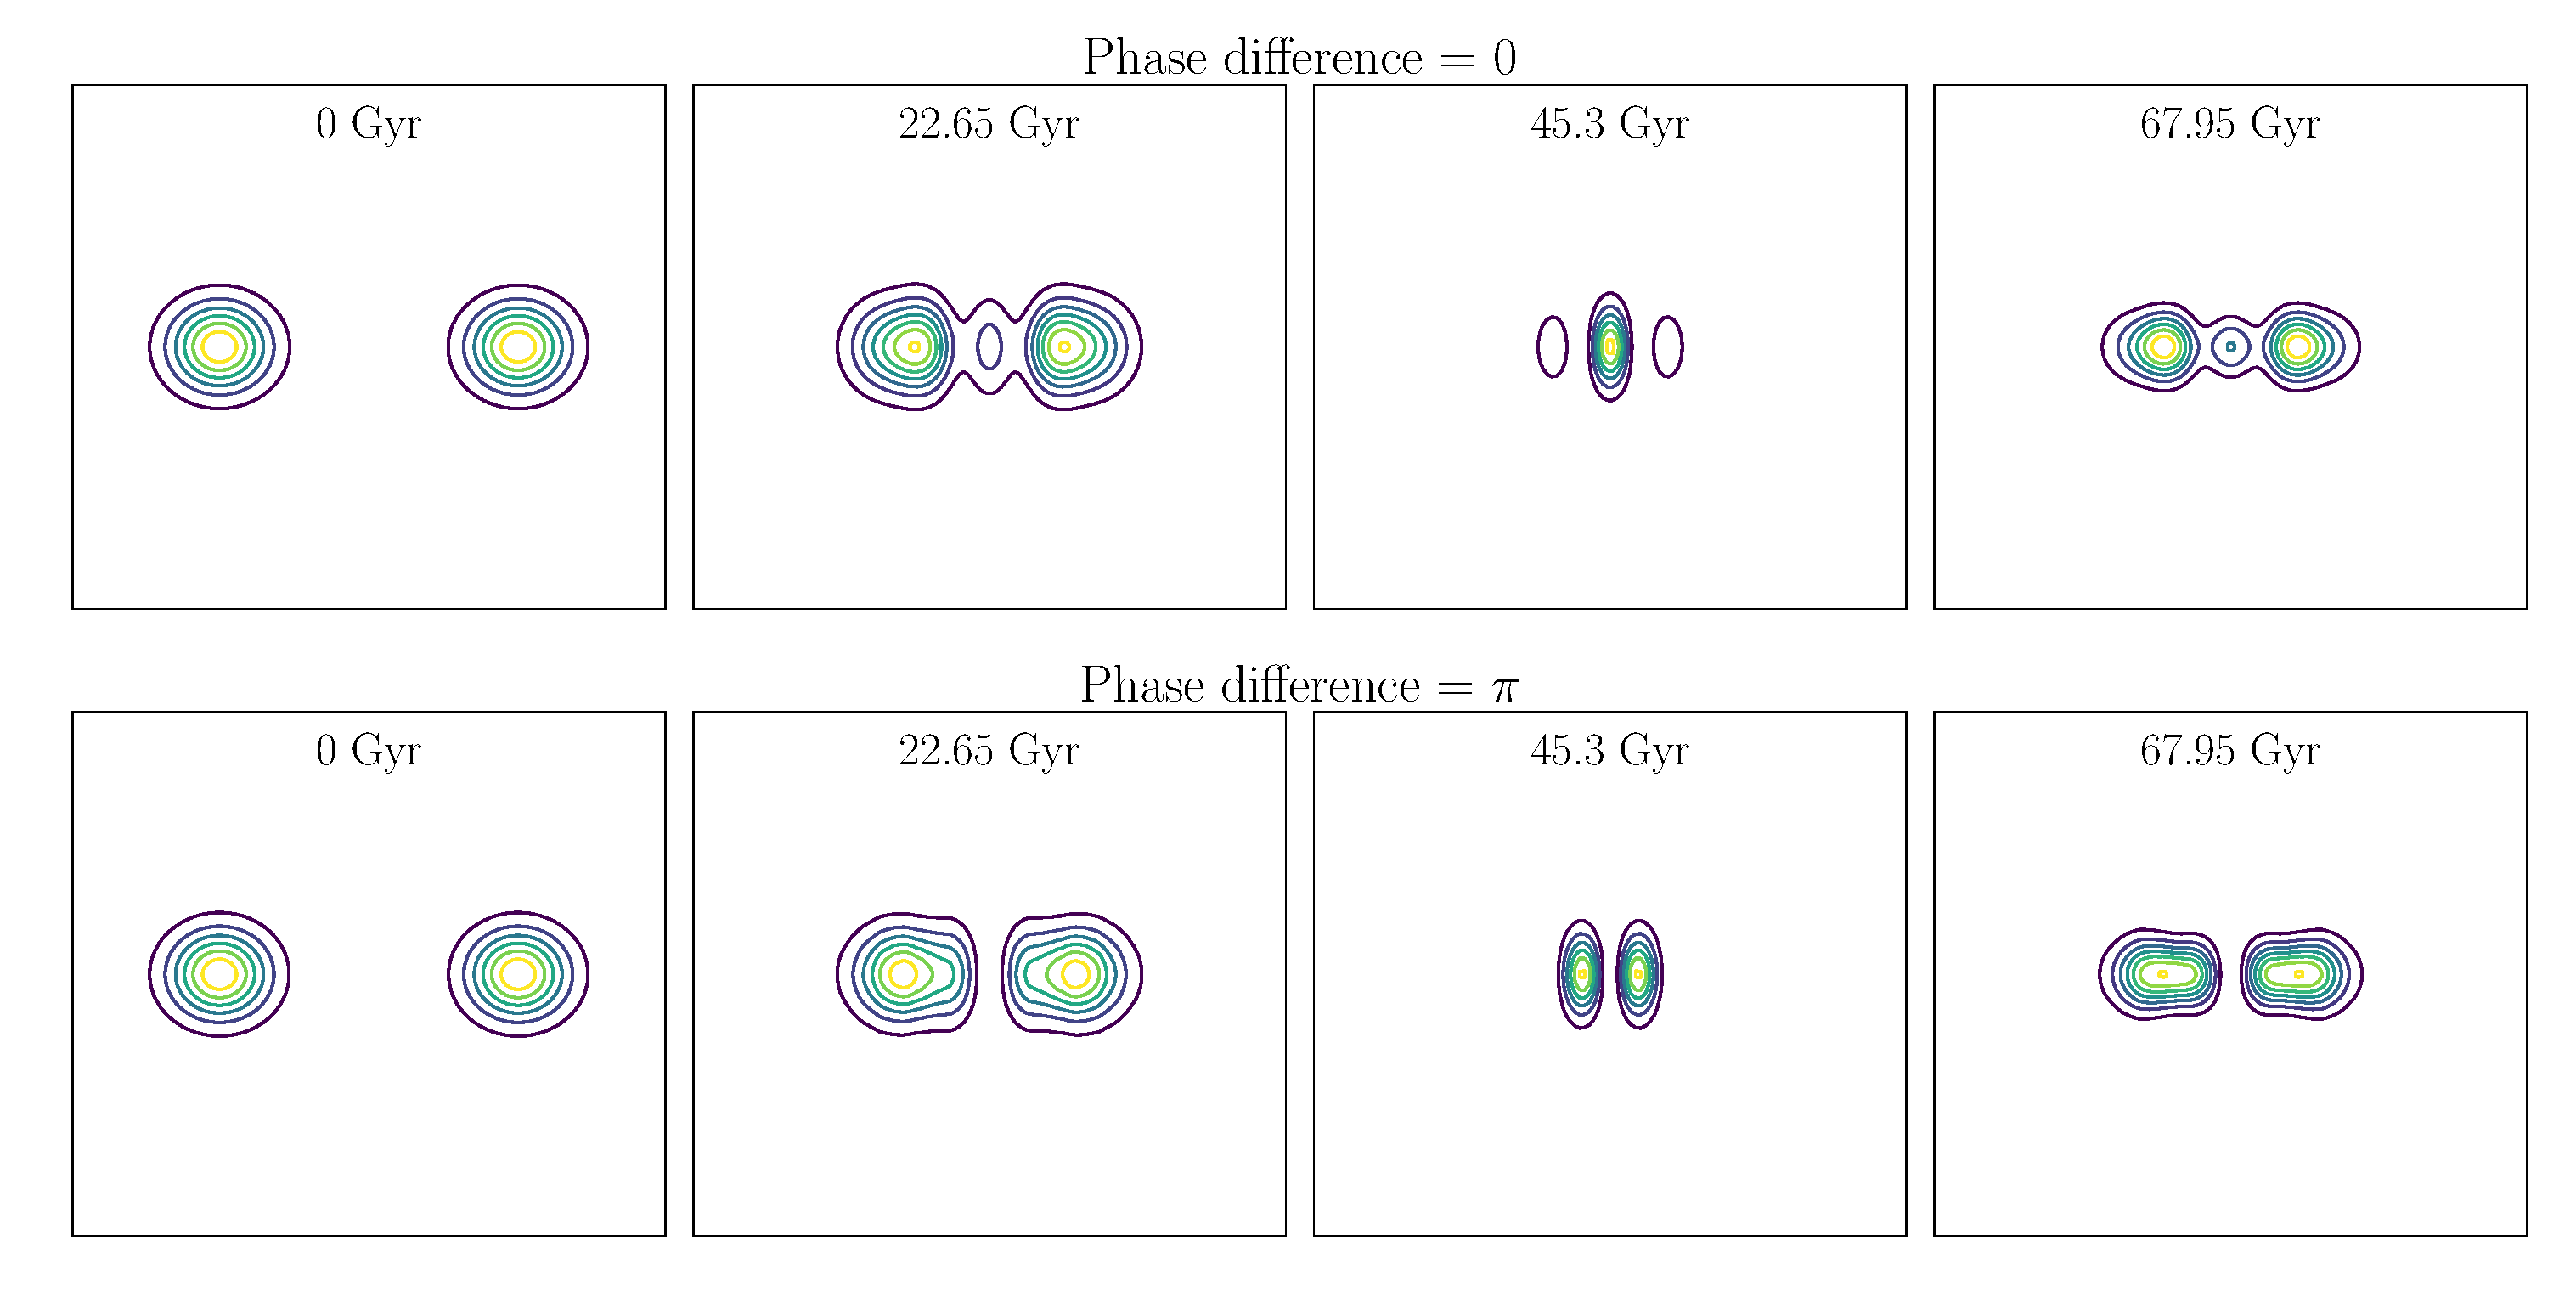
\includegraphics[width=1.\textwidth, trim={0 0 0 0},clip]{phase_comparison}
  \caption{Head-on collisions between two solitons of mass 5, relative velocity 6, and initial separation 4 in code units. Time progresses from left to right across each row.}
  \label{fig:repulsion}
\end{figure}

As demonstrated in \cite{Paredes2016}, the wavelike properties of ULDM can give rise to effective forces which can dramatically affect the dynamics of core collisions. These effective forces arise as a result of interference phenomena, and do not require the ULDM model to incorporate explicit local interactions. Figure \ref{fig:repulsion} shows the results of two simulations using \PyUltraLight in which two solitons of equal mass undergo a head-on collision. Contours of the density profile along the plane of symmetry are displayed. In the first simulation, there is no phase offset between the initial solitons, while in the second simulation the phases differ by $\pi$. We can see that the result of this phase shift is to create an effective repulsive force between the two solitons as they approach one another. Further discussion of this phenomenon and its possible observational consequences can be found in \cite{Paredes2016}.


\vspace{1em}

\subsection{Tidal Disruption of Solitons Orbiting a Central Potential}\label{sec:disruption}

\begin{figure}
  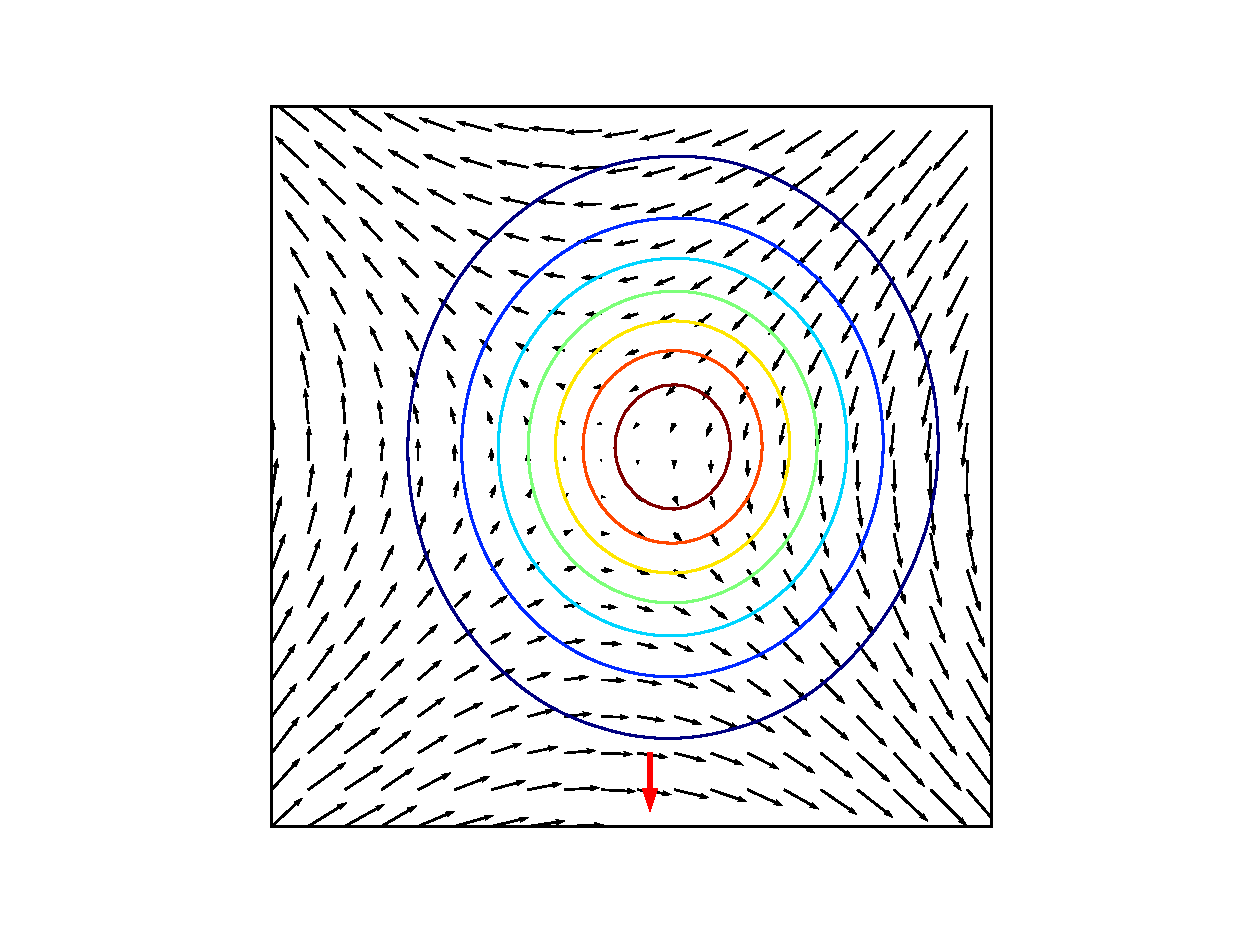
\includegraphics[width=1.\textwidth,trim=1cm 1cm 0 1cm,clip]{riemann}
  \caption{Solitonic core after one revolution of a central potential, demonstrating the internal velocity field of an irrotational Riemann-S ellipsoid (where the collective motion of the soliton has been subtracted from the velocity field). Deformation of the spherical density profile into that of an ellipsoid can be seen, with extension along the radial direction (red arrow).}
  \label{fig:riemann}
\end{figure}

\PyUltraLight is designed such that a central potential may be included by way of a point-mass located at the centre of the simulation grid. While this setup is somewhat unphysical, it provides a starting point for a study of the stability of satellite dark matter halos orbiting a much larger object. Studies of this type can be used to make predictions regarding the lifespans of satellite galaxies around the Milky Way, offering a potential resolution of the so-called missing satellites problem \cite{Weinberg2015}.

An extensive study of the tidal disruption of ULDM solitonic cores orbiting a central potential has recently been undertaken in \cite{Du2018}. Here, we reproduce just one of their results as an additional validity check for \PyUltraLight. In particular, we reproduce the characteristic internal velocity field of a tidally-locked soliton orbiting a central potential. 

When the SP system is recast as a system of hydrodynamical equations, the fluid velocity is given by the gradient of the smoothly-varying phase at any point. This implies that the velocity flow of the SP system is irrotational, $\nabla\times\vec{v}=0$. When a soliton is initialised in a circular orbit around a Newtonian potential, the initially spherical profile is distorted, elongated along the radial direction of the central potential. Meanwhile, the velocity field corresponding to the overall orbital motion of the soliton is superposed with the internal velocity field, combining so as to produce a net flow with vanishing curl. The family of Riemann-S ellipsoids describe uniformly rotating bodies which satisfy the condition of irrotationality \cite{Chandrasekhar1965}, and it is therefore the characteristic internal velocity field of such an ellipsoid which we expect to arise during the simulation. It is found in \cite{Du2018} that an initially spherical solitonic core without self-rotation will gradually spin up to form a tidally-locked irrotational Riemann-S ellipsoid when orbiting a host mass. We are able to reproduce this result using \PyUltraLight, with Figure \ref{fig:riemann} showing the internal velocity field of a solitonic satellite after one complete revolution around a host mass, obtained using \PyUltraLight on a $256^3$ simulation grid. In this case the ratio of host to satellite mass was $\approx 55$. It can be seen that the soliton has become elongated along the radial line connecting to the host, indicating that it is tidally locked. Meanwhile the internal velocity field can be seen to be that of an irrotational Riemann-S ellipsoid \cite{Daller2012}.


%\vspace{1em}

\subsection{Energy Conservation}\label{sec:energy}

\begin{figure}
  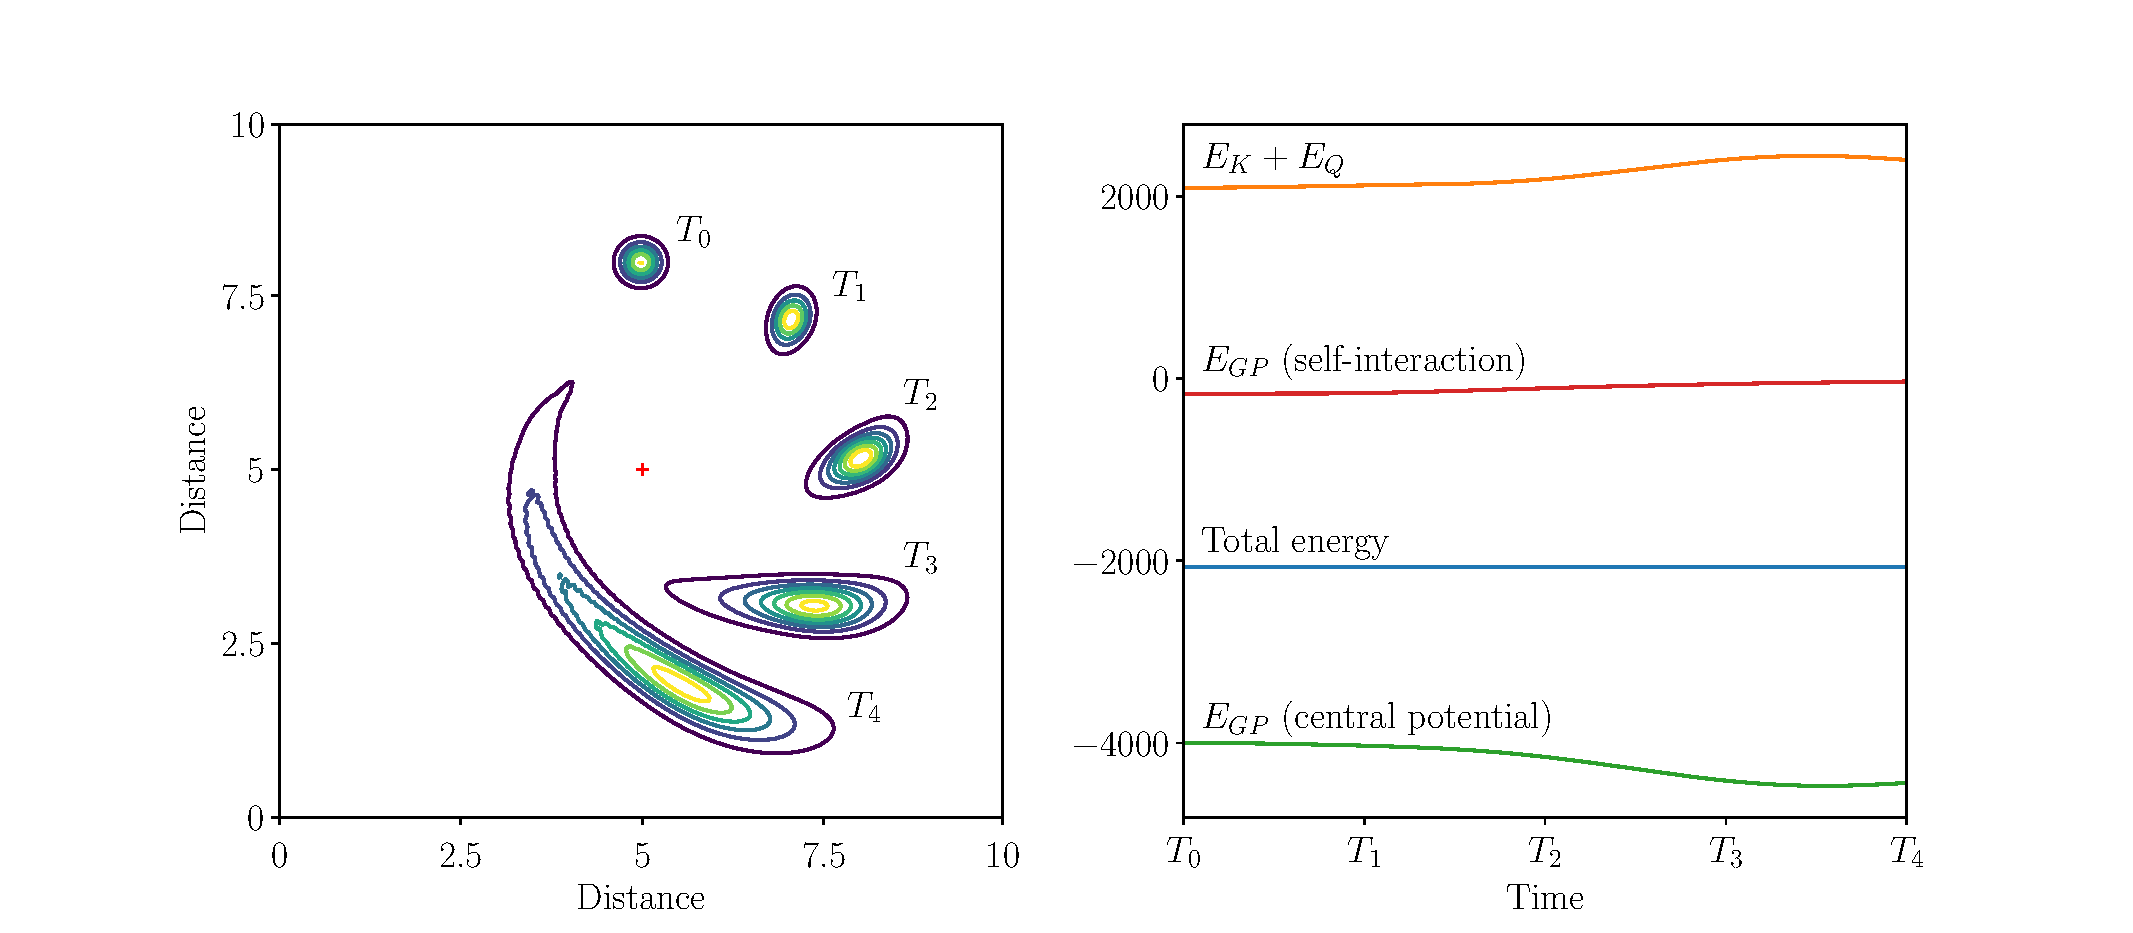
\includegraphics[width=1.1\textwidth,trim=2.5cm 0 0 1cm,clip]{combined_energy_and_density1}
  \caption{Left: Evolution of the density profile of a solitonic core at equally spaced times as it undergoes tidal disruption in a potential centred at the red cross. Right: Evolution of the energy of the system, where times are indicated in correspondence with the snapshots of the density profile. All quantities are in dimensionless code units.}
  \label{fig:combined_1}
\end{figure}

\begin{figure}
  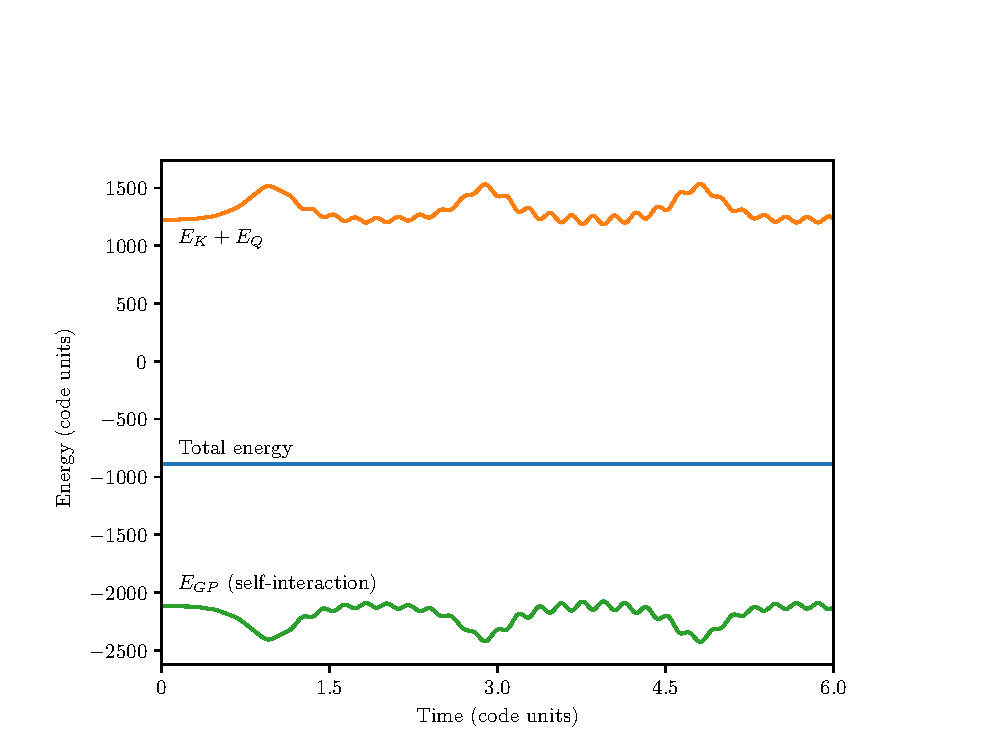
\includegraphics[width=0.9\textwidth,trim=0 0 2cm 2cm,clip]{egy_m=22.eps}
  \caption{Evolution of the energy for a binary soliton system with each soliton in an elliptical orbit around the common centre of mass.}
  \label{fig:binary}
\end{figure}

\begin{figure}
  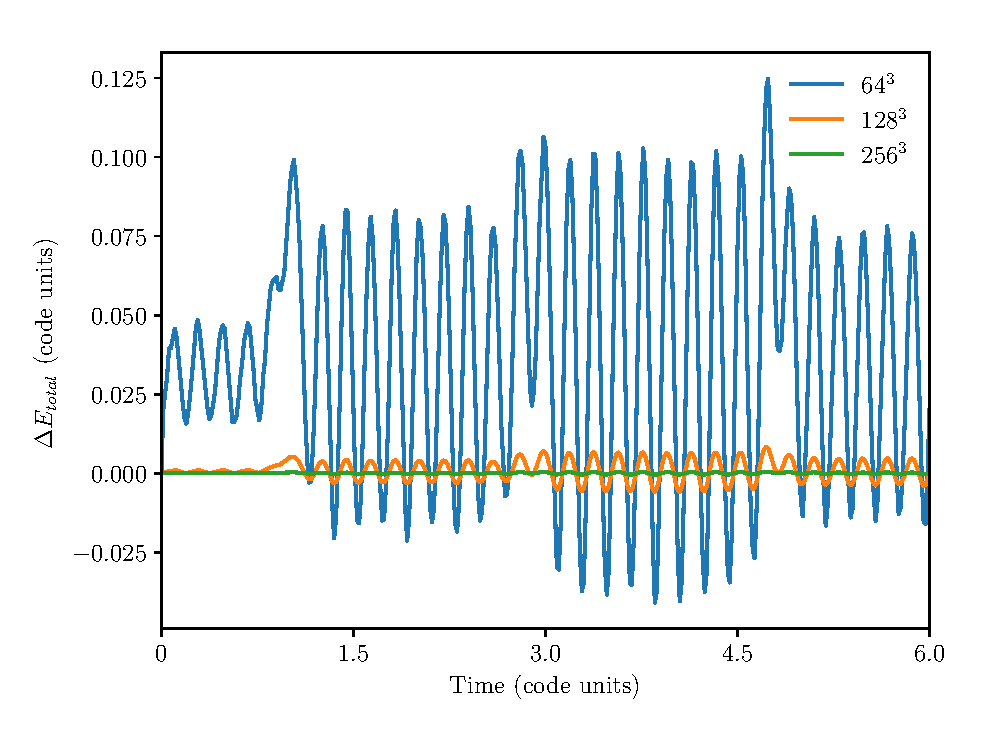
\includegraphics[width=0.9\textwidth,trim=0 0.5cm 0 0,clip]{Total_Energy_Change.eps}
  \caption{Demonstration of improving energy conservation with simulation resolution for a binary system of solitons orbiting their common centre of mass.}
  \label{fig:energy_change}
\end{figure}

In addition to the evolution of the condensate wavefunction $\psi$ and the potential $\Phi$, \PyUltraLight also evaluates the energy of the SP system. An important achievement of the code is sub-percent level energy conservation, even at relatively low spatial resolution, for all dynamical scenarios tested. In this section we derive the expression for the total energy of the SP system and discuss its decomposition into individual constituents calculated separately within the code. We then present the numerical energy evolution of a variety of configurations. 

We begin by defining a suitable action which yields the full SP system through its corresponding Euler-Lagrange equations. We find that variation of
\begin{equation}\label{eq:sp-action}
    S=\int dt\int_{\mathbb{R}^3} d^3x \  -\bigg\{\frac{1}{2}\vert\nabla\Phi\vert^2+\Phi\vert\psi\vert^2+\frac{1}{2}\vert\nabla\psi\vert^2+\frac{i}{2}(\psi\Dot{\psi}^*-\Dot{\psi}\psi^*)\bigg\}
\end{equation}
with respect to $\Phi$, $\psi^*$ and $\psi$ yields equations \ref{eq:p-adim}, \ref{eq:s-adim}, and the conjugate of equation \ref{eq:s-adim}, respectively. The integrand of equation \ref{eq:sp-action} is the Lagrangian density, $\mathcal{L}$, from which we can derive the conserved energy in the usual way:
\begin{equation}
    E_{tot}=\int_{\mathbb{R}^3}d^3x \ \bigg\{\frac{\partial \mathcal{L}}{\partial \Dot{\psi}}\Dot{\psi}+\frac{\partial \mathcal{L}}{\partial \Dot{\psi}^*}\Dot{\psi}^*+\frac{\partial \mathcal{L}}{\partial \Dot{\Phi}}\Dot{\Phi}-\mathcal{L}\bigg\}.
\end{equation}
Evaluating this expression, we obtain:
\begin{align}
    E_{tot}&=\int_{\mathbb{R}^3}d^3x \ \bigg\{\frac{1}{2}\vert\nabla\Phi\vert^2+\Phi\vert\psi\vert^2+\frac{1}{2}\vert\nabla\psi\vert^2\bigg\}\\
    &=\int_{\mathbb{R}^3}d^3x \ \bigg\{\frac{1}{2}\nabla(\Phi\nabla\Phi)-\frac{1}{2}\Phi\nabla^2\Phi+\Phi\vert\psi\vert^2+\frac{1}{2}\nabla(\psi^*\nabla\psi)-\frac{1}{2}\psi^*\nabla^2\psi\bigg\}\\
    &=\int_{\mathbb{R}^3}d^3x \ \bigg\{\frac{1}{2}\Phi\vert\psi\vert^2-\frac{1}{2}\psi^*\nabla^2\psi\bigg\}.\label{eq:energy-tot}
\end{align}
where in the last step we have used Stokes' Theorem as well as the Poisson equation (\ref{eq:p-adim}) to perform simplifications. Because we are working with the dimensionless quantities defined in equation \ref{eq:dimensionless}, it is easy to see that this quantity is related to the physical energy through multiplication by a constant factor of $\CMcal{L}^5\CMcal{T}^{-4}G^{-1}$. It should be noted that equation \ref{eq:energy-tot} is not equivalent to the expectation value of the Schr{\"o}dinger Hamiltonian, which is itself not a conserved quantity of the SP system and is given by
\begin{equation}
    \langle\hat{H}\rangle=\int_{\mathbb{R}^3}d^3x \ \bigg\{\Phi\vert\psi\vert^2-\frac{1}{2}\psi^*\nabla^2\psi\bigg\}.
\end{equation}

The two terms in the integral \ref{eq:energy-tot} are calculated separately within the code. It is easy to see that the first term represents the gravitational potential energy of the SP system. As discussed in \cite{Hui2016}, the second term may be decomposed further into two contributions which may be considered separately as kinetic and `quantum' energies, but for the purposes of this implementation it is sufficient to consider only their combined contribution. Because \PyUltraLight provides the option to include the central potential of a point mass located at the centre of the simulation grid, we have additional energy contributions when such a potential is included. Because this central potential does not arise from a ULDM object, we calculate the gravitational potential energy due to self-interaction separately from the gravitational potential energy due to the central potential.

Figures \ref{fig:combined_1} and \ref{fig:binary} demonstrate energy conservation for two example simulation scenarios. In the first case, we examine the evolution of the energy for a single soliton undergoing significant tidal disruption within a Newtonian central potential. For this simulation a soliton of mass 12 in code units was initialised at a radial distance of 3 code units from the centre of a Newtonian central potential generated by a central mass of 1000 code units. We see that as the soliton is disrupted, the kinetic energy increases, while the gravitational energy due to the central potential decreases, as expected. Meanwhile, the gravitational potential energy due to self-interaction gradually increases toward zero as the disruption continues. The sum of the individual energy components is conserved to $10^{-2}\ \%$ in this case, where the simulation was run at $256^3$. Higher grid resolutions result in even better energy conservation. 

Figure \ref{fig:binary} demonstrates the evolution of the energy of a binary system of solitons in elliptical orbits around their common centre of mass. In this case the simulation ran for approximately three orbital periods at $256^3$. In dimensionless code units, the soliton mass was 22, the initial separation was 2, and the initial relative velocity was 3.6. At points of closest approach, it can be clearly seen that the kinetic energy increases as the solitons speed up, while the potential energy due to self-interaction decreases commensurately such that the total energy is conserved. In this scenario no central potential has been included, so the gravitational energy due to the central potential stays uniformly zero throughout the simulation and is not plotted in the Figure. It can also be seen that as the solitons reach the first point of closest approach, they become slightly deformed, exciting oscillatory modes which are manifest in the Figure as small scale oscillations superposed on the global behaviour. In this case the total energy is conserved to $10^{-3}\ \%$.

Figure \ref{fig:energy_change} demonstrates the relationship between the total integrated energy and the grid resolution for the same binary system of solitons used to generate Figure \ref{fig:binary}. While energy is conserved at sub-percent level even for low resolutions ($96^3$), this is dramatically improved at higher grid resolutions. 


\section{Discussion and Outlook}

We have demonstrated that \PyUltraLight is an accurate tool for the study of the dynamics of ultralight dark matter governed by the Schr{\"o}dinger-Poisson system of equations. The code makes use of a pseudospectral symmetrised split-step Fourier methodology, in which all spatial derivatives are treated via explicit multiplication in the Fourier domain, thereby avoiding difficulties associated with finite-differencing methods. 

Energy conservation within \PyUltraLight is excellent, at sub-percent level for simulations run at $128^3$, and even better performance as resolution is increased. The code is able to reproduce complex phenomena resulting from the wave-like properties of ultralight dark matter as predicted by theoretical models, such as the interference patterns arising during high-velocity collisions of solitonic cores, and the effective forces observed in cases where the colliding cores are out of phase. These phenomena can be clearly observed at relatively low spatial resolution, obviating the need for high-performance computing infrastructure to study the fundamental behaviour of ULDM systems. This makes \PyUltraLight a useful tool for predicting the overall dynamics of a ULDM system in a computationally efficient manner prior to a rigorous examination using more advanced codes such as Nyx.

\PyUltraLight is Python-based, and as such is particularly simple to understand and use. The accompanying Jupyter notebook allows for the efficient adjustment of simulation parameters, and offers a useful browser interface for quick visualisation of simulation results. Despite being Python-based, the code makes use of low-level language resources, namely the FFTW libraries through the use of the Pythonic pyFFTW wrapper. 

While the current implementation of \PyUltraLight is already a useful tool for simulating dynamical ULDM systems, there remains scope for substantial improvement. In particular, it is anticipated that future releases may incorporate adaptive mesh refinement capabilities and variable timestep functionality. Additionally, while the current implementation utilises a spatial grid of fixed size and does not provide a means by which to incorporate baryonic density contributions, future releases are likely to allow for cosmic expansion and a means by which to incorporate simplified models of baryonic matter. Further adaptations of the code may also be implemented to allow for greater flexibility in the choice of ULDM model, incorporating possibilities such as explicit self-interaction. 





\appendix
\section{Download and Licensing}

\PyUltraLight has been made publicly available under a BSD licence. The full code repository, including supplementary files such as the code used to generate soliton profiles, is available on GitHub at https://github.com/erckendall/PyUltraLight. \PyUltraLight makes use of the pyFFTW pythonic wrapper around the FFTW C-based fast Fourier transform libraries. Both pyFFTW and FFTW are freely-available. \PyUltraLight has been successfully tested on both Mac OS and Linux operating systems, though not exhaustively. The current version of \PyUltraLight, as demonstrated in this work, is capable of reproducing many of the results of previous ULDM simulations, and we plan to extend its capabilities in future releases.  

\acknowledgments

TBW



% The bibliography will probably be heavily edited during typesetting.
% We'll parse it and, using the arxiv number or the journal data, will
% query inspire, trying to verify the data (this will probalby spot
% eventual typos) and retrive the document DOI and eventual errata.
% We however suggest to always provide author, title and journal data:
% in short all the informations that clearly identify a document.

%\section*{References}
\bibliographystyle{JHEP-mod}
\bibliography{refs} 


%\begin{thebibliography}{99}

%\bibitem{a}
%Author, \emph{Title}, \emph{J. Abbrev.} {\bf vol} (year) pg.

%\bibitem{b}
%Author, \emph{Title},
%arxiv:1234.5678.

%\bibitem{c}
%Author, \emph{Title},
%Publisher (year).

% Please avoid comments such as "For a review'', "For some examples",
% "and references therein" or move them in the text. In general,
% please leave only references in the bibliography and move all
% accessory text in footnotes.

% Also, please have only one work for each \bibitem.

%\end{thebibliography}

\end{document}
